\documentclass[10pt, letterpaper]{article}
\usepackage[letterpaper, left=2cm, right=2cm, top=2cm, bottom=2cm]{geometry}

\usepackage[english]{babel}
\usepackage{setspace}
\usepackage{graphicx}
% MAKE FONTFACE SANS SERIF
%\renewcommand{\familydefault}{\sfdefault} 
% SELECT FONT TYPE
%\usepackage{avant} %helvet works too


\usepackage[hidelinks]{hyperref}
\hypersetup{
	colorlinks=true,
	linkcolor=red,
	filecolor=magenta,      
	urlcolor=teal,
	pdftitle={An Example},
	%pdfpagemode=FullScreen,	
}

\urlstyle{sf}

\usepackage{booktabs}
\usepackage[table]{xcolor}
\usepackage{tcolorbox}

\def\tecdemty{Tecnol\'ogico de Monterrey, campus Monterrey}
\def\school{Escuela de Ingenier\'ia y Ciencias}
\def\me{Prof. Mat\'ias V\'azquez Pi\~n\'on (\href{mailto:matias.vazquez@tec.mx}{\texttt{matias.vazquez@tec.mx}})}
\def\course{TE2015 Microcontroladores}
\def\doctitle{HW1.2 Case Study: The 8051 Architecture}

\usepackage{tikz}
\usepackage{circuitikz}
\usetikzlibrary{calc}

\begin{document}
\noindent
	\begin{tabular}[b]{@{}l@{}}
	{\bfseries\Large\tecdemty}\\ [1mm]
	{\bfseries\large\school}\\ [5mm]
	{\bfseries\large\course}\\ [1mm]
	{\bfseries\large{\doctitle}}\\ [1mm]
	{\large\me} \\ [1mm]
	{\large Due date: \href{https://experiencia21.tec.mx/courses/286463/assignments/9678285}{Friday, August 19}} \\ [1mm] 

\end{tabular}	\hfill
\includegraphics[height=1.3in]{img/logoTec.eps}

\section*{General Purpose Input/Output}
\subsection*{Introduction}
\href{https://en.wikipedia.org/wiki/Intel_8051}{INTEL’s 8051} is an 8-bit microcontroller architecture developed in 1981 and \href{https://www.digikey.com.mx/es/products/filter/integrados-microcontroladores/685?s=N4IgjCBcoKwAwDYqgMZQGYEMA2BnApgDQgD2UA2iAEwAcCAnFXCALrEAOALlCAMqcAnAJYA7AOYgAvtKA}{still found in the marked today}. One of the currently available microcontrollers based on the 8051 architecture is \href{https://en.wikipedia.org/wiki/Atmel_AT89_series}{ATMEL’s AT89C51}, which datasheet can be \href{http://ww1.microchip.com/downloads/en/devicedoc/doc4383.pdf}{found online}. In this case study, we will go over some of the 8051’s features using the AT89C51 device. Notice that some other devices that share similar architecture can be also found in the market. 

According to Figure 1 (page 8) of the AT89C51AC3 microcontroller datasheet, ports 1, 3 and 4 share similar structure, which is shown below:

\begin{center}
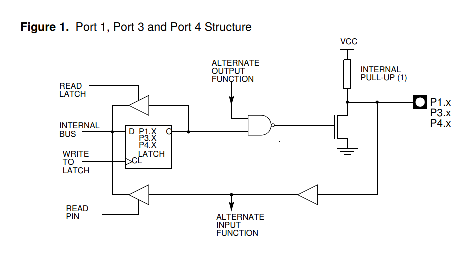
\includegraphics[width=0.65\textwidth]{img/fig01.eps}
\end{center}

To drive a logic level (0 or 1) as an output of ports 1, 3 and 4, some conditions must be accomplished, as follows (see pin description table on pages 5-7 on the datasheet for further reference):
\begin{enumerate}
\item The signal to output is held by INTERNAL BUS and should follow the path towards P1.x, P3.x or P4.x
\item To this to happen, first the LATCH must drive the signal in its input, D, (connected to INTERNAL BUS) towards Q with a clock pulse (CL)
\item Once the INTERNAL BUS signal is transferred to the LATCH output, Q, it is used as one of two inputs of a NAND gate. 
\item The second input of the NAND gate is a signal called ALTERNATE OUTPUT FUNCTION. According to the truth table of a NAND gate, if the value of this signal is 0, the output is set to 1 (highlighted in grey in the table below); however, if the value of ALTERNATE OUTPUT FUNCTION is 1, the output of the gate is the inverted value of Q, so is the inverted value of INTERNAL BUS. 

\begin{table}[h!]
	\begin{center}
		\begin{tabular}{| c c | c |}
			\hline
			Q (from Fliop-Flop) & ALTERNATE OUTPUT FUNCTION & OUTPUT \\
			\hline
			0 & 0 & 1 \\
			0 & 1 & 1 \\
			1 & 0 & 1 \\
			1 & 1 & 0 \\
			\hline
		\end{tabular}
	\end{center}
	\caption{Truth table of the two-input NAND gate.}
\end{table}

\item In this sense, to allow the value of INTERNAL BUS to pass through the NAND gate, ALTERNATE OUTPUT FUNCTION must be set to 1, at the expense that the value to output is inverted.
\item Following the signal path, the output of the NAND gate is used to turn ON (with logic 1) or OFF (with logic 0) the Field Effect Transistor (FET), as it is connected to its Gate terminal. This means that if the value of INTERNAL BUS is 0, the FET’s Gate logic value is set to 1, turning ON the transistor; and if INTERNAL BUS is 1, the FET’s Gate logic value is 0, turning the transistor OFF.
\item If the FET is OFF, an open circuit can be assumed between the FET’s Source and Drain pins, so the pull-up resistor connected between the FET’s Source and VCC pulls the pin voltage (P1.x, P3.x or P4.x) up to a logic 1 (hence the name, pull-up resistor). In the opposite case, if the FET is ON, a short circuit is assumed between Source and Drain, driving the pin P1.x, P3.x or P4.x value to a logic 0 (by shorting the pin to ground) and the VCC voltage is entirely absorbed by the pull-up resistor. This means, that the value at INTERNAL BUS is inverted again by the pull-up resistor.  
\item This way, the value of INTERNAL BUS value is transferred from the internal data bus of the microcontroller to any pin of ports P1, P3 or P4 as soon as ALTERNATE OUTPUT FUNCTION is set to 1, as shown in the table below:

\begin{table}[h!]
	\begin{center}
		\begin{tabular}{| c c | c |}
			\hline
			INTERNAL BUS & ALTERNATE OUTPUT FUNCTION & P1.x, P3.x or P4.x \\
			\hline
			0 & 0 & 0 \\
			0 & 1 & 0 \\
			1 & 0 & 0 \\
			1 & 1 & 1 \\
			\hline
		\end{tabular}
	\end{center}
	\caption{Truth table of ports P1, P3 and P4.}
\end{table}
\end{enumerate}

\emph{\textbf{Note:}} Ports P1, P3 and P4 count on a pull-up resistor (a resistor connected between \texttt{VCC} and \texttt{Drain} of driving FET) to force the logic \texttt{1} to \texttt{VCC} level when the FET is off.

\subsection*{Activity}
\begin{enumerate}
\item On the same fashion, describe the path followed by the value of INTERNAL SIGNAL towards P0.x (see Figure 2 of the datasheet). Note that in this case, there is no pull-up resistor pulling the output value to \texttt{VCC} for a logic \texttt{1}; instead, a FET is used, which is turned on only when both \texttt{ADDRESS LOW/DATA} and \texttt{CONTROL} signals are high. This is called a \emph{strong pull-up}. However, strong pull-ups of \texttt{P0} and \texttt{P2} can only be used when these ports are configured as memory buses (\texttt{CONTROL = 1}) and not as a GPIO (\texttt{CONTROL = 0}), thus in the latter case, \texttt{P0.x} and \texttt{P2} exhibit an open drain output when a logic 1 set on \texttt{INTERNAL BUS}.

\begin{center}
	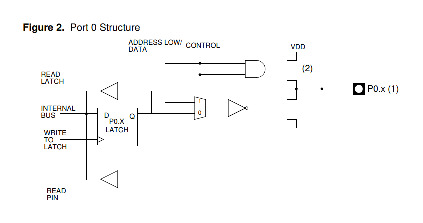
\includegraphics[width=0.7\textwidth]{img/fig02.eps}
\end{center}

Complement your description with a truth table that shows the change at \texttt{P0.x} depending on \texttt{INTERNAL BUS}, \texttt{ADDRESS LOW/DATA} and \texttt{CONTROL} signals (i.e., \texttt{ADDRESS LOW/DATA} is one same signal which switches functions to output a memory address or data depending of the port configuration.)

\item Continue with your analysis of the 8051 GPIO but now describe the path followed by the value of INTERNAL SIGNAL towards \texttt{P2.x} (Figure 3 of the datasheet). Complement your description with a truth table that shows the change at \texttt{P2.x} depending on \texttt{INTERNAL BUS}, \texttt{ADDRESS HIGH/DATA} and \texttt{CONTROL} signals.
\begin{center}
	\includegraphics[width=0.7\textwidth]{img/fig03.eps}
\end{center}

\item Considering that ports \texttt{P0} and \texttt{P2} exhibit open drains when operating as GPIO for the logic \texttt{1} case, what do you propose to achieve a logic \texttt{1} instead of an open drain when working with GPIO in this configuration?
\end{enumerate}
\end{document}
